\documentclass[aspectratio=169,10pt]{beamer}
\usetheme{Madrid}
\usecolortheme{default}

\usepackage[utf8]{inputenc}
\usepackage[T1]{fontenc}
\usepackage{amsmath,amssymb}
\usepackage{booktabs}
\usepackage{graphicx}
\usepackage{listings}
\usepackage{hyperref}

\definecolor{unibblue}{RGB}{0,51,102}
\definecolor{unibgold}{RGB}{212,175,55}
\definecolor{unibgreen}{RGB}{0,128,0}
\definecolor{codebg}{RGB}{244,247,251}

\setbeamercolor{structure}{fg=unibblue}
\setbeamercolor{palette primary}{bg=unibblue,fg=white}
\setbeamercolor{palette secondary}{bg=unibblue!85,fg=white}
\setbeamercolor{palette tertiary}{bg=unibblue!70,fg=white}
\setbeamercolor{block title}{bg=unibblue!90,fg=white}
\setbeamercolor{block body}{bg=unibblue!8,fg=black}
\setbeamercolor{alertblock title}{bg=unibgold!90,fg=black}
\setbeamercolor{alertblock body}{bg=unibgold!14,fg=black}
\setbeamercolor{exampleblock title}{bg=unibgreen!85,fg=white}
\setbeamercolor{exampleblock body}{bg=unibgreen!8,fg=black}

\lstset{
  language=Python,
  basicstyle=\ttfamily\scriptsize,
  backgroundcolor=\color{codebg},
  frame=single,
  rulecolor=\color{unibblue!35},
  keywordstyle=\color{unibblue}\bfseries,
  commentstyle=\color{unibgreen!80!black}\itshape,
  showstringspaces=false,
  breaklines=true
}

\title[Aliran Daya Python — Modul 4]{Analisis Aliran Daya Menggunakan Python}
\subtitle{Modul 4: Kontinjensi $N-1$, Proyek Capstone \& Peta Jalan Seri Level 2}
\author[Novalio Daratha]{Novalio Daratha\\Program Studi Teknik Elektro, Universitas Bengkulu}
\date{Workshop Teknis Intensif (32 JP) — 2026}

\begin{document}

\begin{frame}
  \titlepage
\end{frame}

\begin{frame}{Agenda Modul 4 (8 JP)}
  \tableofcontents
\end{frame}

\section{Kriteria Keamanan $N-1$ \& Indeks Keparahan ($PI$)}

\begin{frame}[fragile]{Kriteria Keamanan $N-1$ \& Skrining Cepat Bebas \texttt{deepcopy}}
  \begin{block}{Indeks Keparahan Komposit ($PI$, Eksponen $2n = 4$)}
    \[
      PI_k = \sum_{l=1}^{N_{\text{br}}} \frac{w_l}{2n}\left(\frac{|S_l|}{S_l^{\text{rated}}}\right)^{2n}
           + \sum_{i=1}^{N_b} \frac{w_{v,i}}{2n}\left(\frac{|V_i| - V_i^{\text{nom}}}{\Delta V_i^{\text{lim}}}\right)^{2n}
    \]
  \end{block}
  \begin{columns}[T]
    \begin{column}{0.54\textwidth}
\begin{lstlisting}
elem_table.at[idx, "in_service"] = False
try:
    work_net.res_bus["vm_pu"] = base_vm.values
    pp.runpp(work_net, algorithm="nr",
             init="results", max_iteration=30)
finally:
    elem_table.at[idx, "in_service"] = True
\end{lstlisting}
    \end{column}
    \begin{column}{0.43\textwidth}
      \begin{alertblock}{Keunggulan Pola \texttt{try...finally}}
        \begin{itemize}
          \item Bebas duplikasi memori \texttt{deepcopy} di dalam loop.
          \item Mencegah kebocoran status (kontinjensi $N-k$ tak disengaja).
          \item \textit{Warm start} memotong jumlah iterasi NR.
        \end{itemize}
      \end{alertblock}
    \end{column}
  \end{columns}
\end{frame}

\section{Hasil Skrining $N-1$ IEEE 14-Bus}

\begin{frame}{Heatmap Pembebanan $21\times 20$ \& Topologi Kontinjensi Terburuk}
  \begin{columns}[T]
    \begin{column}{0.54\textwidth}
      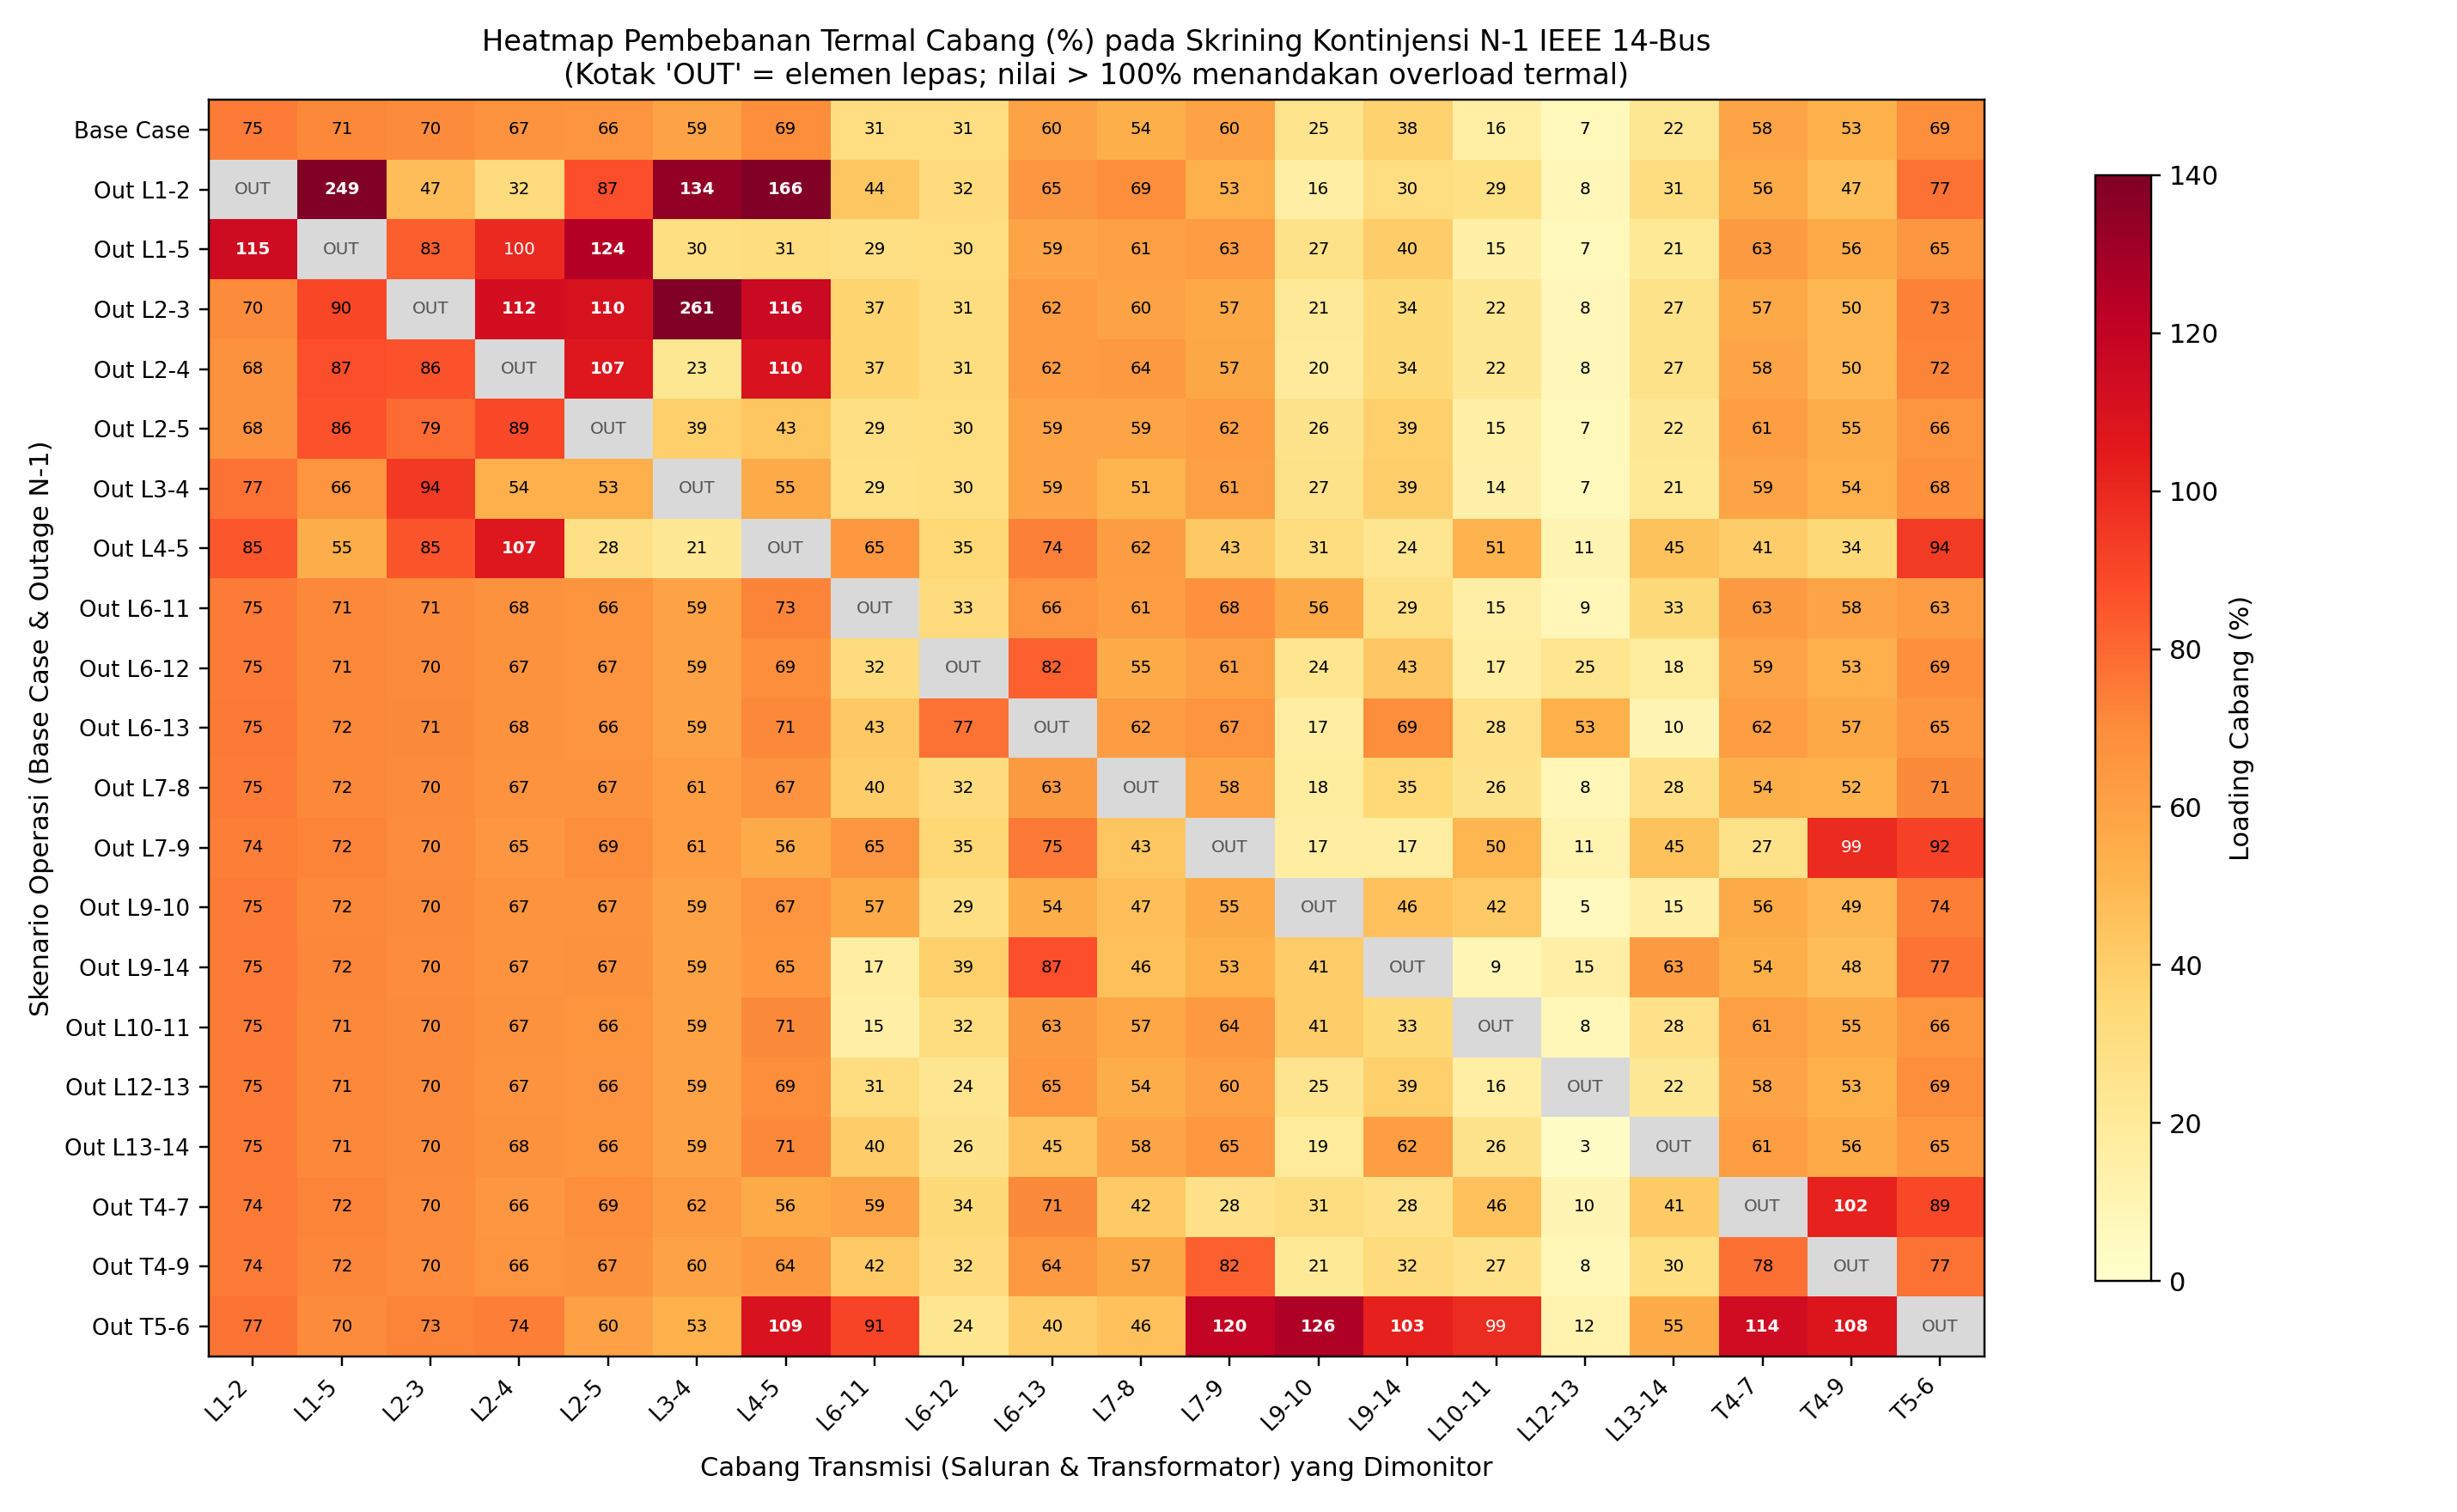
\includegraphics[width=\textwidth]{../figures/n1_line_loading_heatmap.png}
    \end{column}
    \begin{column}{0.44\textwidth}
      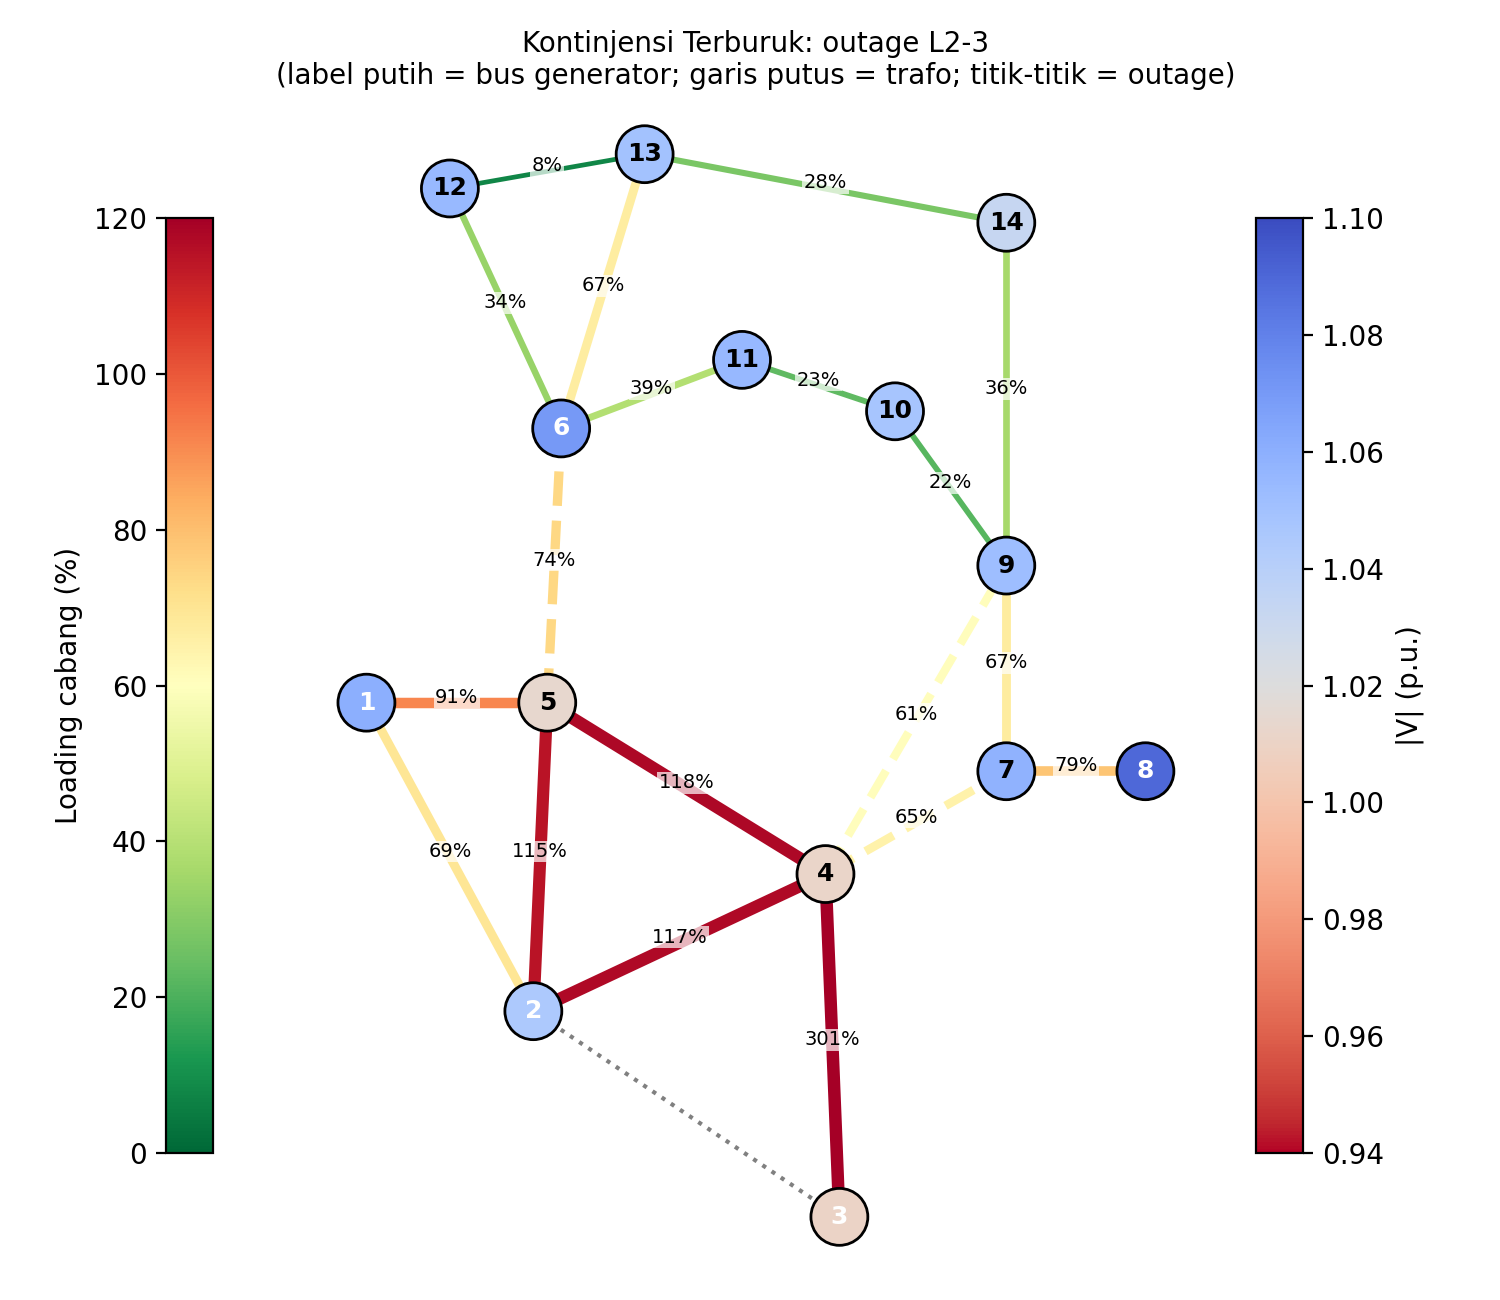
\includegraphics[width=0.92\textwidth]{../figures/topologi_kontinjensi_terburuk.png}
    \end{column}
  \end{columns}
  \vspace{0.1cm}
  \begin{exampleblock}{Temuan Kritis 20 Cabang (17 Saluran + 3 Trafo)}
    \scriptsize
    \textbf{Rank 1: \texttt{L2-3}} ($PI=95{,}5$, \texttt{L3-4} mencapai $301{,}5\%$ MVA / $260{,}8\%$ arus, 4 cabang \textit{overload});
    \textbf{Rank 2: \texttt{L1-2}} ($PI=60{,}1$, \texttt{L1-5} $=251{,}2\%$);
    \textbf{Rank 3: \texttt{T5-6}} ($PI=27{,}0$, 7 cabang \textit{overload});
    \textbf{\texttt{L7-8}}: \textbf{ISLANDING} (Bus 8 terisolasi).
  \end{exampleblock}
\end{frame}

\section{Seri Lanjutan Level 2: OPF, PV Hosting \& Risiko $N-2$}

\begin{frame}{Peta Jalan Level 2 (1): Optimal Power Flow (AC-OPF) \& PV Hosting}
  \begin{columns}[T]
    \begin{column}{0.49\textwidth}
      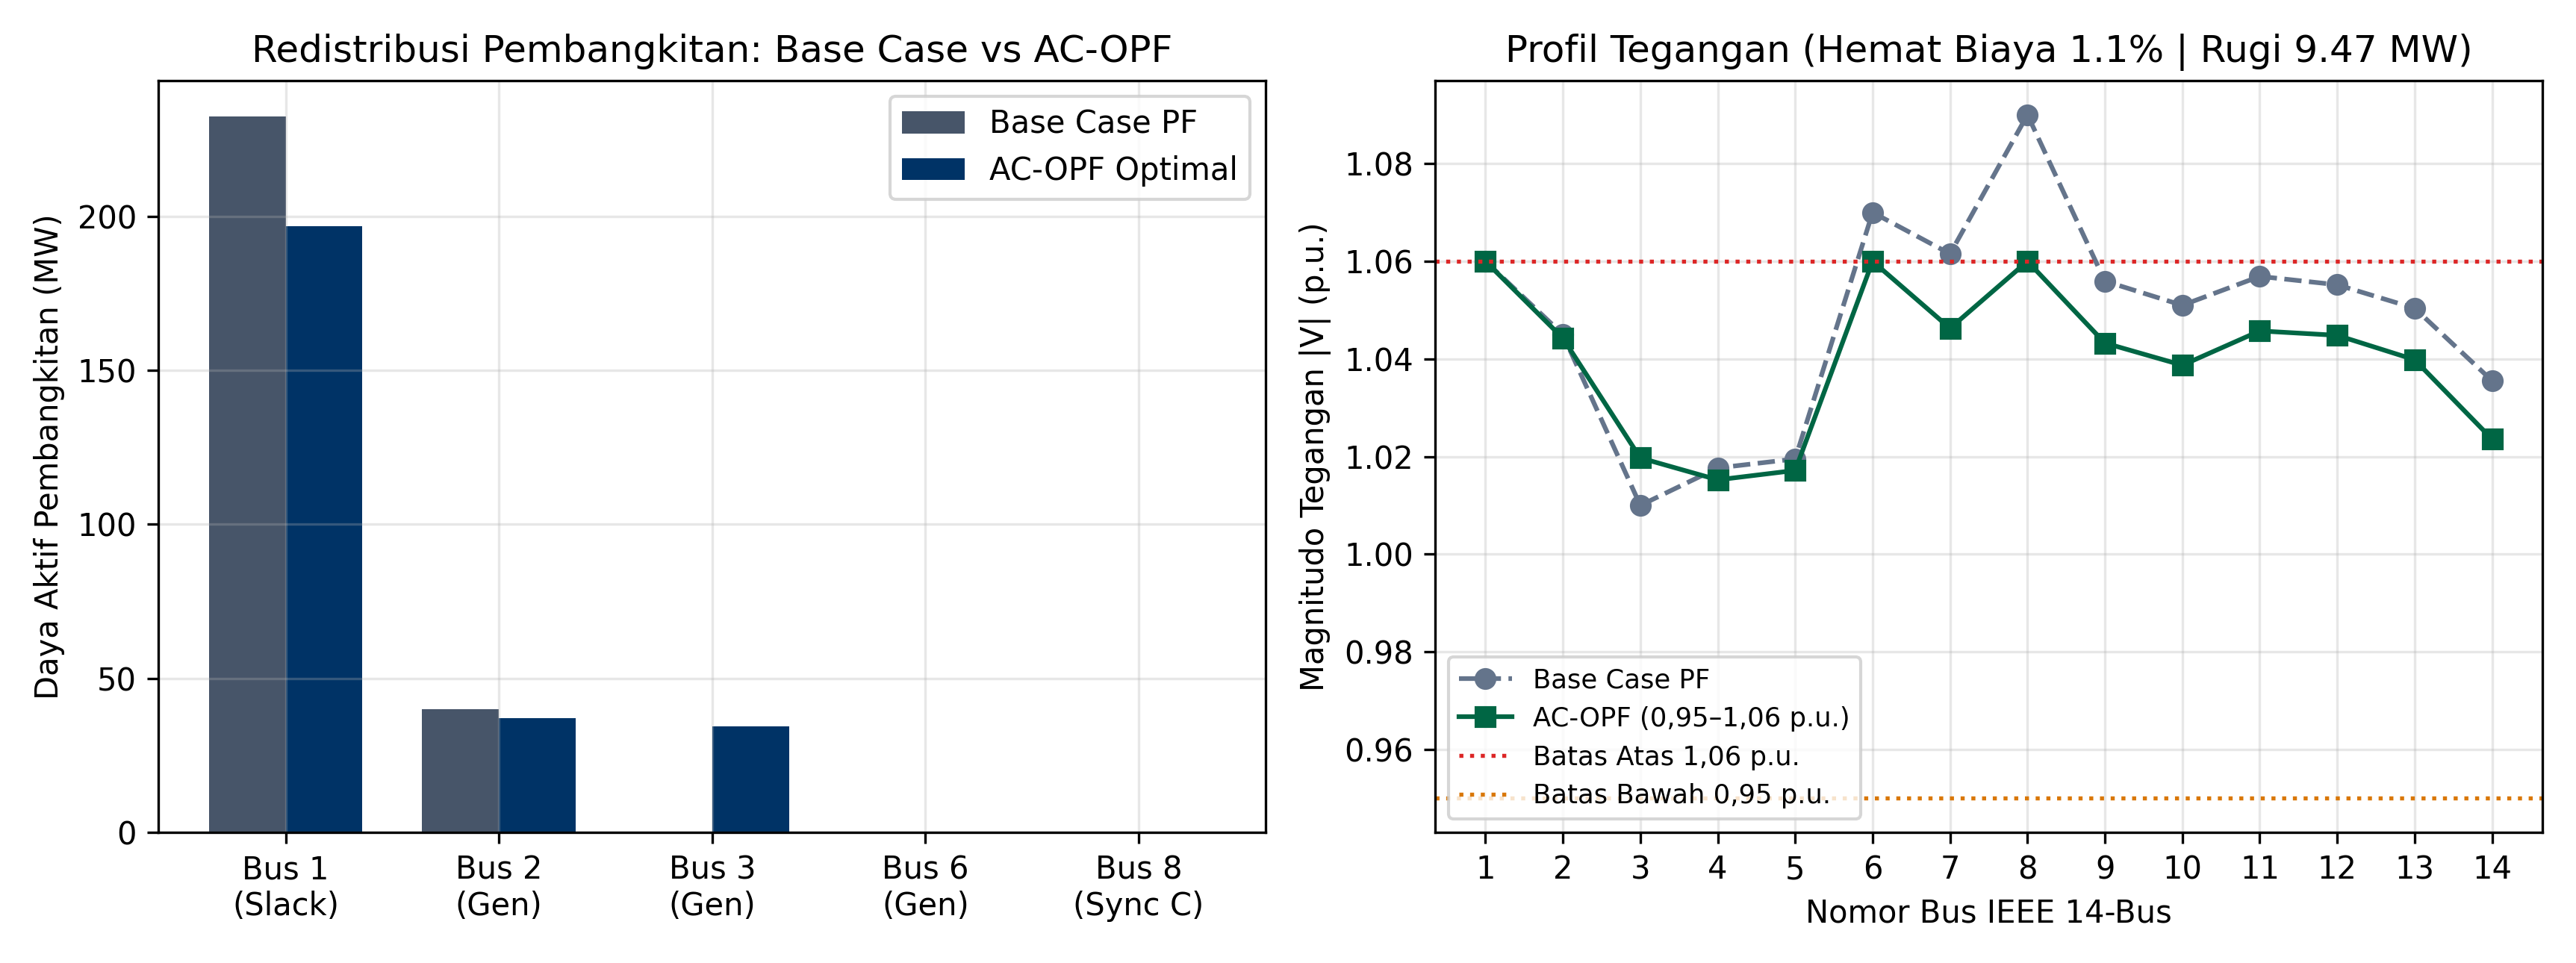
\includegraphics[width=\textwidth]{../figures/level2_opf_comparison.png}
      \begin{block}{Hasil AC-OPF IEEE 14-Bus (\texttt{runopp})}
        \scriptsize
        Biaya turun $\$8.170{,}15 \to \mathbf{\$8.082{,}26/\text{jam}}$ (hemat $1{,}08\%$); rugi transmisi anjlok $13{,}39 \to \mathbf{9{,}47\text{ MW}}$ ($-29{,}3\%$); LMP $\$36{,}92\text{--}\$41{,}52/\text{MWh}$.
      \end{block}
    \end{column}
    \begin{column}{0.49\textwidth}
      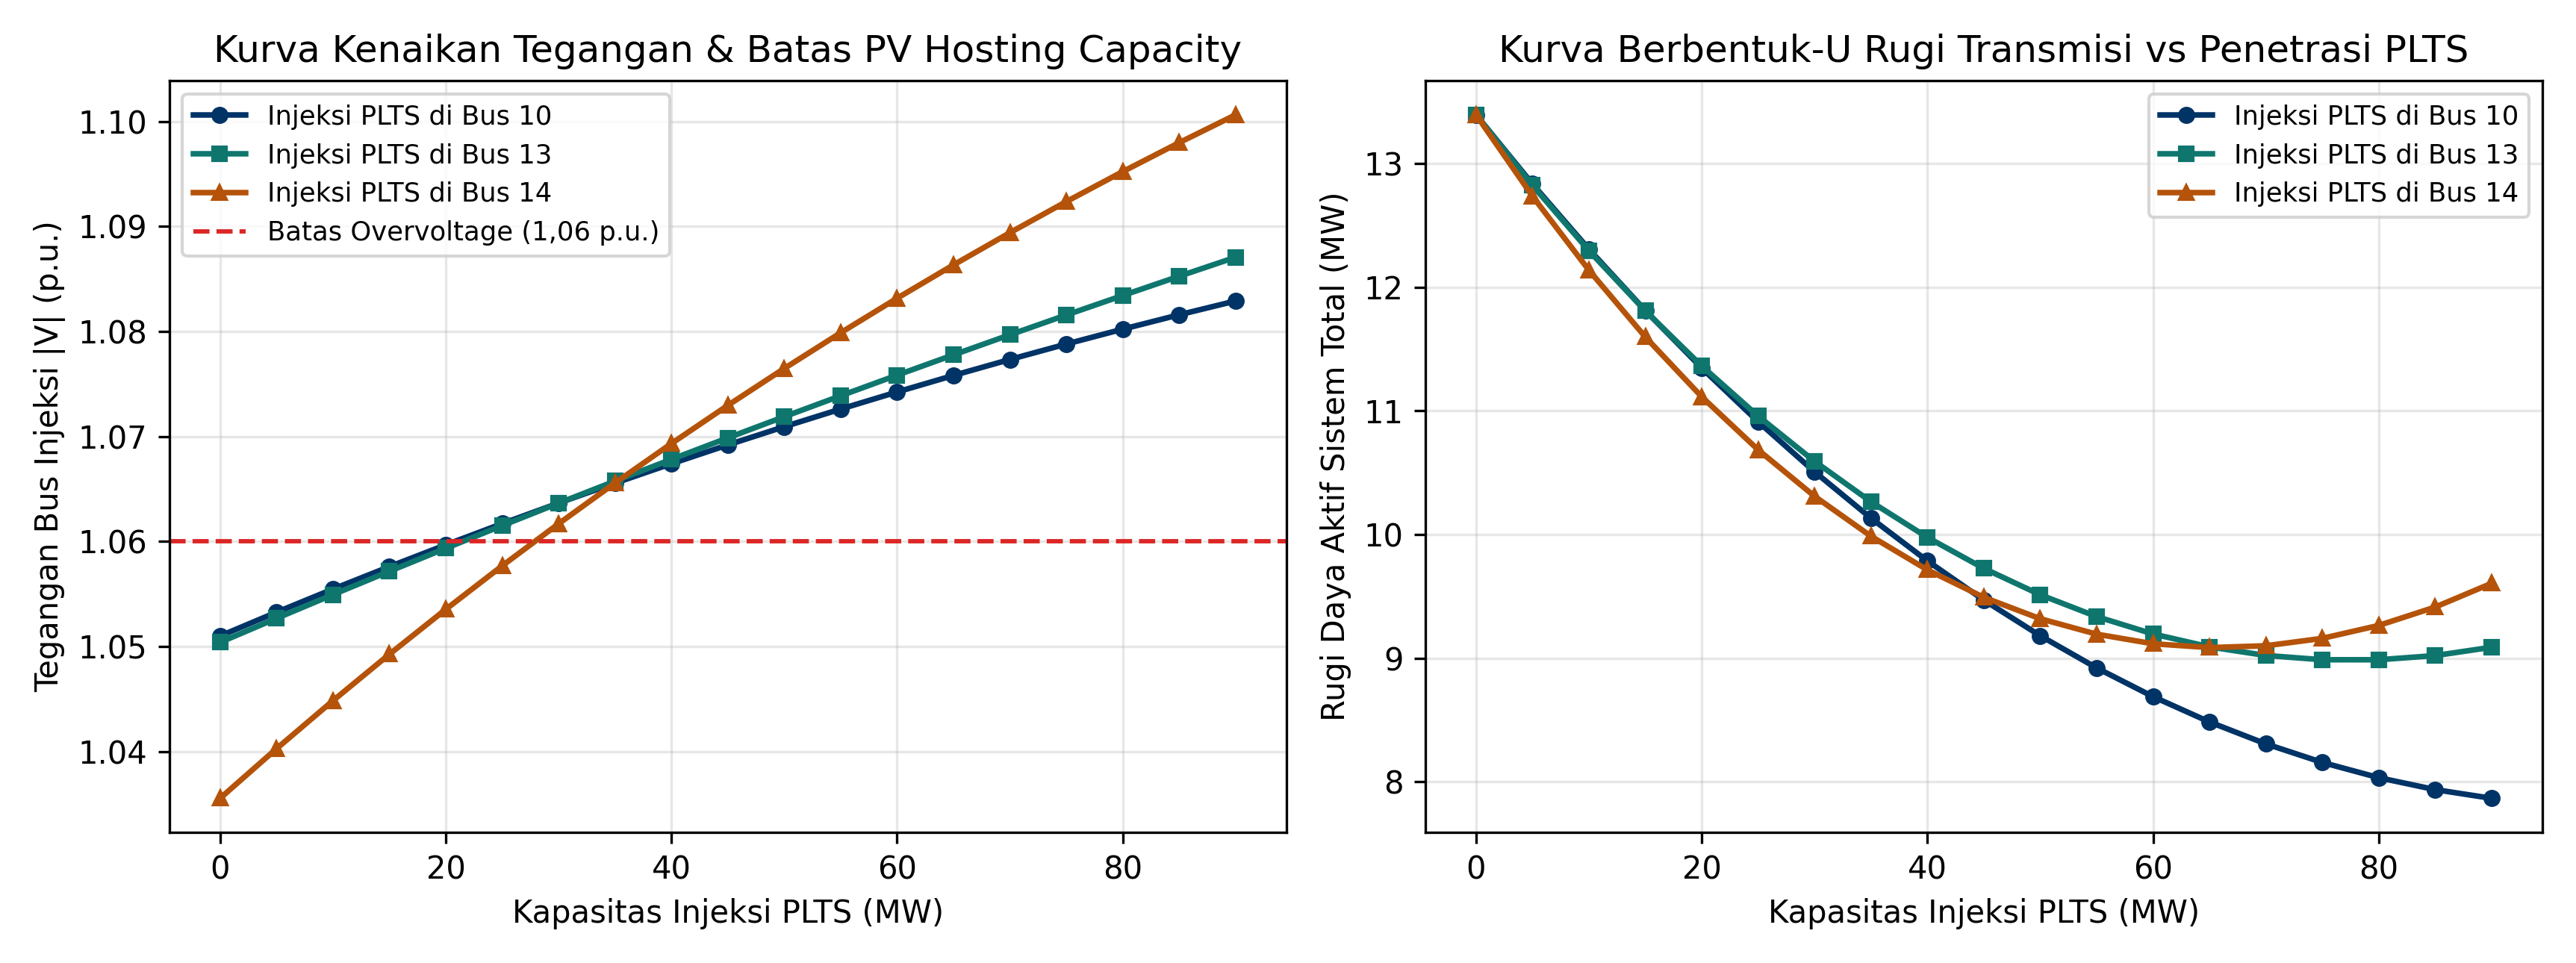
\includegraphics[width=\textwidth]{../figures/level2_pv_hosting_capacity.png}
      \begin{exampleblock}{Kapasitas Hosting PLTS ($|V| \le 1{,}06\text{ p.u.}$)}
        \scriptsize
        Bus 10: \textbf{10 MW}, Bus 13: \textbf{20 MW}, Bus 14: \textbf{25 MW}. Menunjukkan kurva berbentuk-U rugi transmisi terhadap penetrasi EBT.
      \end{exampleblock}
    \end{column}
  \end{columns}
\end{frame}

\begin{frame}{Peta Jalan Level 2 (2): Skrining Kontinjensi Ganda $N-2$ Berbasis Risiko}
  \begin{columns}[T]
    \begin{column}{0.61\textwidth}
      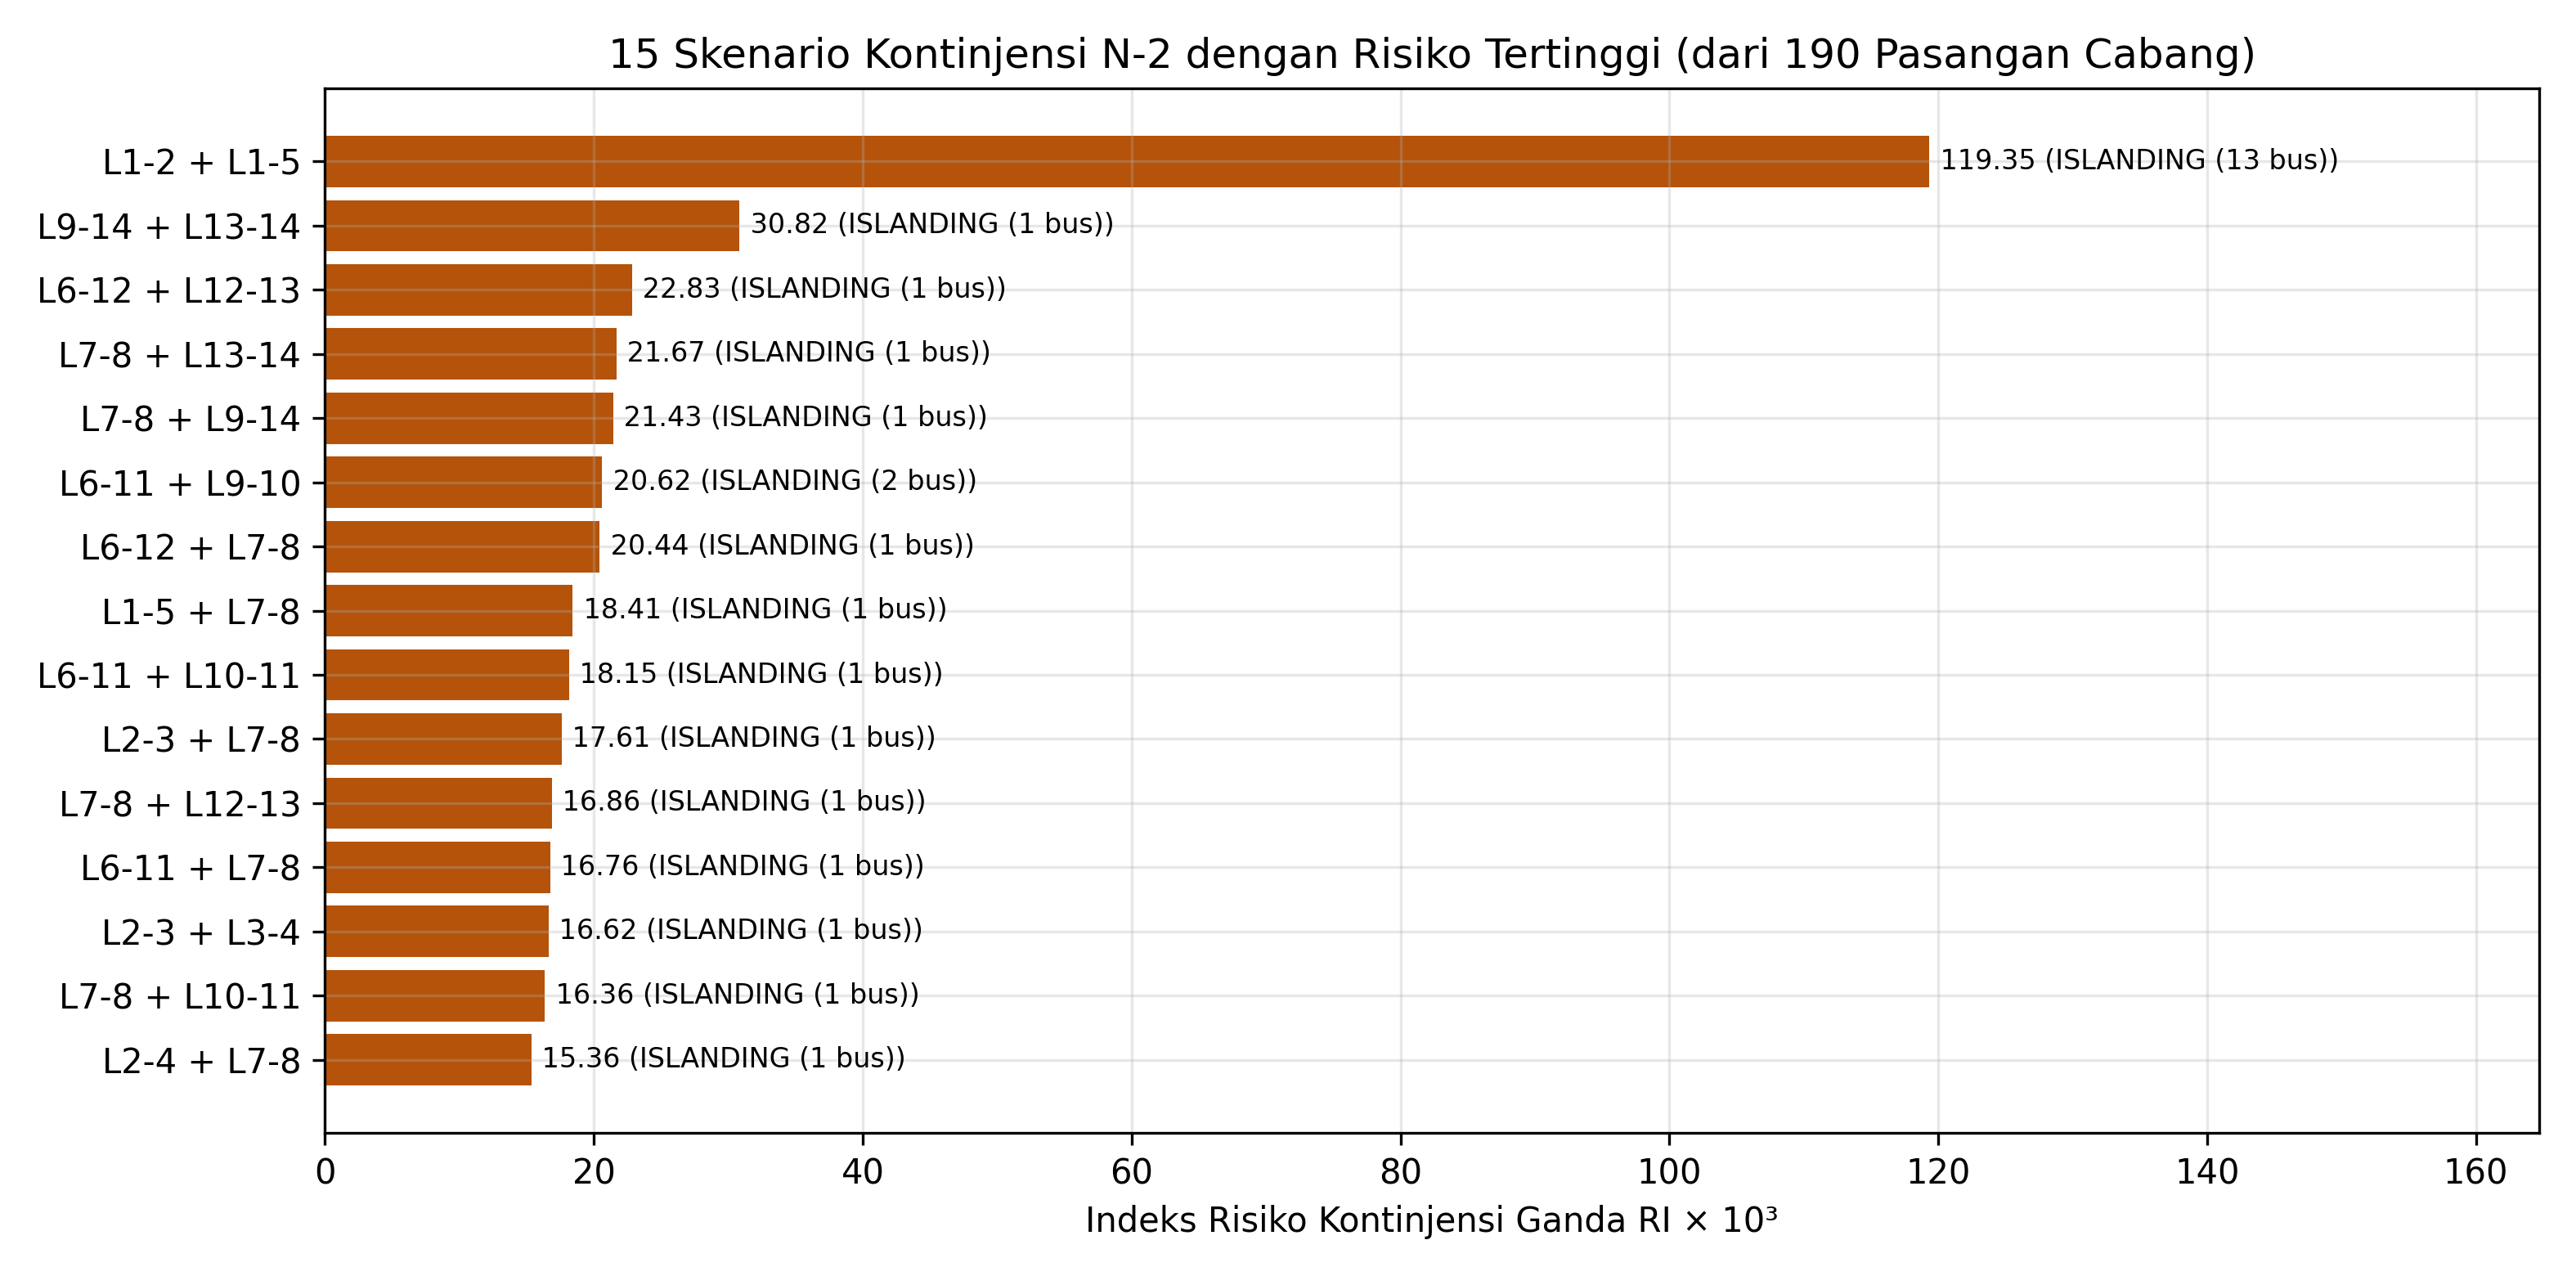
\includegraphics[width=\textwidth]{../figures/level2_n2_risk_top15.png}
    \end{column}
    \begin{column}{0.37\textwidth}
      \begin{block}{Indeks Risiko ($RI_{ij}$)}
        \[
          RI_{ij} = p_i p_j \cdot \left(PI_{S,ij} + PI_{V,ij} + P_{\text{island}}\right)
        \]
      \end{block}
      \begin{alertblock}{Evaluasi 190 Pasangan Cabang}
        \scriptsize
        \begin{itemize}
          \item $\binom{20}{2} = 190$ skenario $N-2$ teruji otomatis.
          \item Terdeteksi \textbf{27 skenario \textit{islanding}}.
          \item Risiko \#1: \texttt{L1-2 + L1-5} (memutus Slack dari 13 bus).
          \item Risiko \#2: \texttt{L9-14 + L13-14} (probabilitas tertinggi, Bus 14 terisolasi).
        \end{itemize}
      \end{alertblock}
    \end{column}
  \end{columns}
\end{frame}

\begin{frame}{Terima Kasih — Siap Menuju Proyek Capstone \& Level 2!}
  \begin{center}
    \vspace{0.7cm}
    {\Large \textbf{Terima Kasih}}\\
    \vspace{0.35cm}
    {\large Eksekusi Level 2: \texttt{python3 level2/level2\_advanced\_studies.py}}\\
    \vspace{1.1cm}
    Novalio Daratha\\
    Program Studi Teknik Elektro, Universitas Bengkulu\\
    \texttt{https://ndaratha.my.id/w-pf/}
  \end{center}
\end{frame}

\end{document}
